\section{Computing and software for particle physics}

Scientific outcomes of an experiment are made possible by the development of an efficient computing and software infrastructure. Historically, the development of these infrastructures for particle physics has benefited from Moore's law, the use of commodity hardware, and highly  distributed systems.  This, however, no longer holds true. Nowadays, the landscape of computing infrastructure for particle physics is rapidly changing and becoming more diverse.  The particle physics community faces important challenges in this area and the current computing and software models must evolve to meet the needs of approved and future experiments. %Presently real challenges are facing HEP and they must be addressed through innovation, long term planning, collaboration, R\&D, software optimization and more. 
%[move this to the Challenges section?] In the meanwhile professional development of staff and trainees in computing and software is called for\cite{ID114}.   


\subsection{Computing challenges of current and next generation experiments, and evolution}
Since early 2000s the particle physics community has adopted a large scale distributed computing model whereby grid technologies integrate computer centers worldwide to form a single computing and storage infrastructure supporting, for example, the LHC experiments~\cite{bib:IB-talk}. At the same time, the use of heterogeneous facilities consisting of cloud computing, HPC and High Level Trigger (HLT) farms has offered extra opportunistic capacity, though often at the cost of significant development effort and suited to a subset of workflows. As a result, presently, the particle physics community has access to an amount of computing resources meeting the needs of its physics programs.
%, as well as Extra opportunistic computation capacity is available. 
 
In the coming years, however, the science programs at the HL-LHC Run 4 and beyond, Belle-II at SuperKEKB, future circular and linear colliders (\FCC, \CEPC, \ILC, \CLIC, etc), and large neutrino experiments (DUNE, JUNO, etc)~[ID126], will together require about an order of magnitude more %$\sim$10 times the 
computing resources presently available, while increase in funding for computing is not expected~\cite{bib:MK-talk}.  For example, Fig.~\ref{fig:atlas-computing} shows the estimated CPU and disk resource needs of ATLAS during LHC Run 4 and beyond~\cite{bib:atlas-computing}.  Within this context, the community faces a number of challenges that needs to be urgently addressed, now, in order to enable the physics outcomes of future experiments. 
\begin{itemize}
\item Cost : Predictability of hardware cost has become difficult as the price trends are driven by commercial markets and the increased performance that was seen for the same amount of money due to Moore's Law no longer holds.  
%Moore's Law meets limitations and the price trends are driven by commercial markets. 
\item Hardware evolution: Computing resources are nowadays becoming increasingly heterogeneous, placing requirements on both the code base and on the experiment computing systems.
\item Data storage, management and preservation: Data storage needs of future projects exceed the predicted capacity and affordability of the current data storage and management model.  The current model also does not provide the adaptability required to efficiently exploit heterogeneous compute infrastructures. 
There is also an uncertainty in the future availability of tape storage which could have significant impact on the data storage capacity available to experiments.  The tape market now depends on a single manufacturer, increasing the risk of market collapse.

\item Software challenges: Large volume of legacy software used in particle physics requires important improvements in memory usage and throughput.  The software must also be upgraded to make the most efficient use of different computing platforms, e.g. to take advantage of increased processing power from accelerators and GPU use, tuning on CPUs, etc. The current legacy software also offers many opportunities for algorithmic enhancement, and should also be upgraded to take advantage of development in machine learning and AI applications.
\item Increase in the skill gap between early career physicists and the profile needed for programming on new compute architectures~[ID114] necessitates the needs for professional training, development and career opportunities for computing-software professionals [ID114, ID53, ID29, ID5, ID127, ID150, ID59, ID64, ID34, ID68, ID69, ID115, ID134, ID163].

%- HEP applications need to be modernized to take advantage of the hardware evolution, and tap more into GPUs.
%- Significant changes are needed to accommodate new architectures and a more heterogeneous computing environment. 

%\item Data volume challenge at the HL-LHC, storage and data management and preservation - data storage needs are hard to fulfill and storage service is challenging to operate. There is a strong need to conduct R\&D activities that will evaluate components and techniques to build a common HEP data cloud;
%\item Expanding the effective use of the heterogeneous facilities - how to strengthen the link between HEP and HPC centers and find effective common and scalable solutions to the challenges of data intensive processing required by the HEP communities; cost effective use of commercial clouds and the associated interfaces, vendor locking, networking and procurement~\cite{ID16, ID53, ID59, ID64, ID77, ID79, ID108, ID127, ID162, ID150};  
%\item HEP software challenges - software is probably the biggest opportunity to address the possible future HEP storage of computing resources~\cite{ID79,ID53,ID162,ID5,ID150,ID126,ID16,ID34,ID43,ID127,ID114,ID101,ID134,ID163}. Migrate and improve large volume of legacy HEP software to optimize the memory usage and throughput, to increase the processing power from GPU use and tuning on CPUs and algorithmic enhancement and to take advantage development in machine learning and AI applications. To implement a radical change in this aspect a multi-year planning and multi-collaboration and institutional commitment will be needed.
%\item Increase in the skill gaps between early career physicists and profile needed for programming on the new architectures~\cite{ID114} necessitates the needs for professional training, development and career opportunities for computing-software professionals~\cite{ID114, ID53, ID29, ID5, ID127, ID150, ID59, ID64, ID34, ID68, ID69, ID115, ID134, ID163}.
%\item Quantum computing and other revolutionary technologies~\cite{ID162,ID150, ID59,ID128,ID88,ID148,ID157} – even though quantum computing is probably in the far future, HEP community can begin to consider ways to adopt HEP software to the data format and the architecture of the future quantum computers. 
\end{itemize}


\begin{figure}
    \centering
    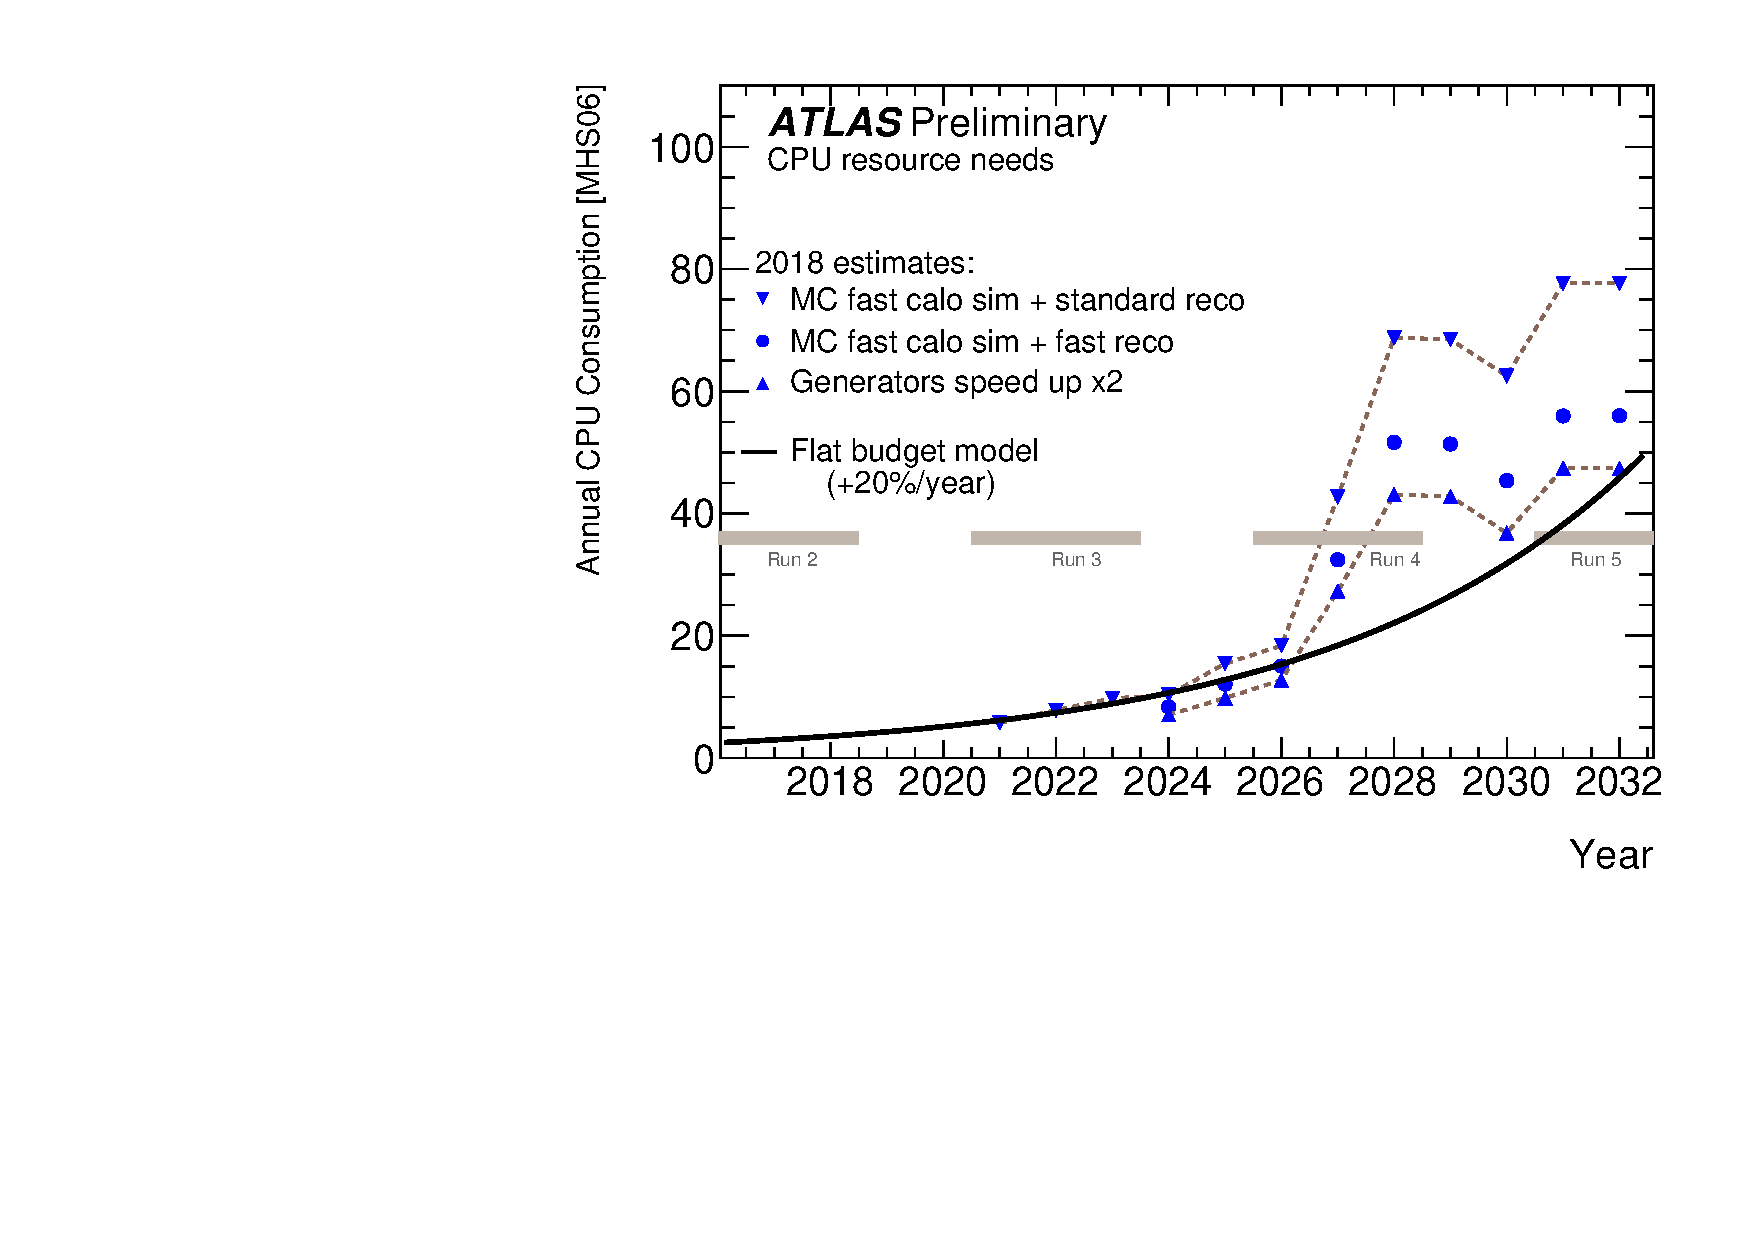
\includegraphics[width=0.49\textwidth]{Instrum/img/ATLAS-cpu-HL-LHC.pdf}\hfill
    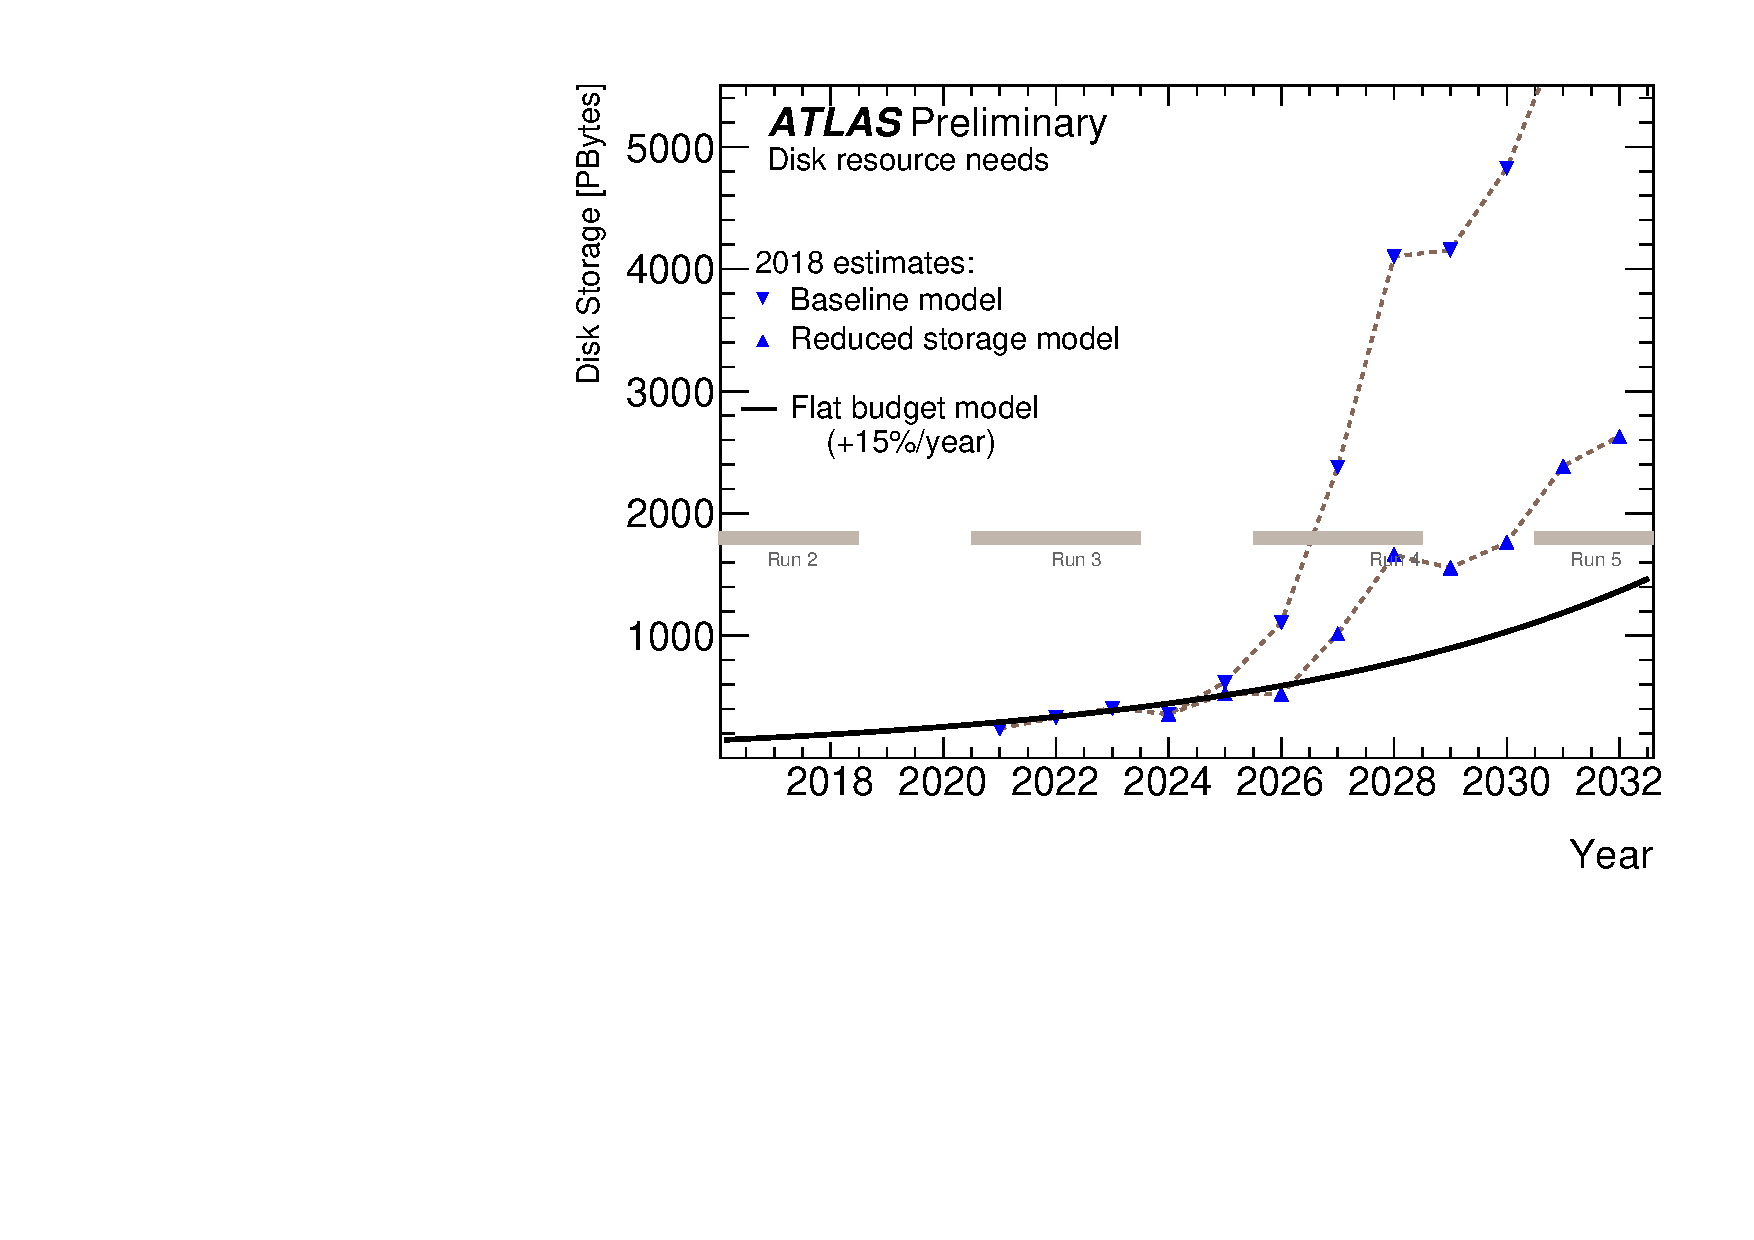
\includegraphics[width=0.49\textwidth]{Instrum/img/ATLAS-disk-HL-LHC.pdf}
    \caption{Estimated CPU (left) and total disk resources (right) needed by the ATLAS experiment as a function of time for both data and simulation processing.  Plots taken from~\cite{bib:atlas-computing}.
    }
    \label{fig:atlas-computing}
\end{figure}

As approved projects enter into operation and future projects are being developed, it is clear that there will be unprecedented pressure on computing resources availability for particle physics in the 2020s. 
Past experience has shown that development timescales are long, and therefore, these challenges must be addressed now to maximize the scientific outputs of tomorrow.  


\subsection{R\&D for computing and software}

To meet the challenges laid out in this document, the particle physics community must carry out carefully planned and coordinated R\&D programs~[ID53, ID79, ID162, ID5, ID127, ID150, ID64, ID84, ID117, ID126, ID134] that will adopt new hardware, take advantage of industrial trends and emerging technologies, improve the software, and position HEP computing and software for the revolutionary and disruptive technologies. Past experience has shown that it is important to plan, from the start, the development of an agile computing and software infrastructure, as technologies will continue to evolve~\cite{bib:RJ-talk}.  It is also equally important to plan for an infrastructure that requires less hardware and less effort to maintain and operate as an experiment matures~\cite{bib:RJ-talk}. The following highlights areas of R\&D activities that must be pursued~\cite{bib:MG-talk,bib:GS-talk}.

\begin{itemize}
    \item Tools and applications development for effective use of capacity provided by heterogeneous hardware and specialized architectures.
    For example, these include tools and applications to take advantage of
    GPU improvements for extremely parallel applications that offload the demand on CPUs, to provide workflow and task specific acceleration, to enable pattern recognition and data transformation with FPGAs, to provide a cost effective way to enhance the memory bandwidth and low power consumption with TPUs\footnote{Tensor Processing Unit -- an ASIC accelerator for AI applications.}, and to provide common provisioning mechanisms transparent to users.
    %----
    \item Application and data access tools development at HPC facilities and using commercial clouds, which can deliver extra capacity to particle physics.  
    
    \item Continued R\&D on data organization, infrastructure, management and access in the face of technological changes and cost increase due to large data volume, data preservation and the data open access requirement~[ID150, ID77, ID79]. 
 
    \item Software R\&D, which is expected to provide one of the biggest opportunities to address the needs of the particle physics community.  While inefficiently designed software is very costly in terms of resource usage, good and clever software allows greater physics opportunities within the same fixed resource budget.  For the HL-LHC experiments, the software and the data formats will be improved to allow for more efficient processing and storage. To best use the technologies, algorithms and HEP software need to be redesigned and written, respectively. Common software framework, turnkey stacks can be developed through the inter-experiment collaboration for the HL-LHC and future collider projects. There are great opportunities for HEP to improve and generate new software by organizing the community, reaching out to industry, software engineers and other sciences~[ID53, ID79, ID162, ID150, ID126, ID16, ID34, ID43, ID127, ID162, ID77, ID59, ID64, ID108].
    
    \item Hardware infrastructure development and support. The particle physics community should seize the opportunity to be involved in the planning stage of future multidisciplinary research infrastructures, such as large HPC systems and Clouds (e.g. European Open Science Cloud (EOSC)), in order to ensure that these systems will be best equipped to address the needs of the community.  Likewise, the maintenance of existing, and development of new, computing centers for HEP is expected to continue to be important.
    
    
    \item Preparation and follow-up for the innovative, new technologies on the horizon, such as quantum computing and neuromorphic computing~[ID59, ID128].  These may revolutionize HEP computing, despite the fact that they have a great deal of uncertainties. The particle physics community must position itself to be able to migrate seamlessly to the new technology when it is ready.

\end{itemize}

To effectively carry out the above activities, the field needs more skilled developers, and a significant investment here is required~[ID5, ID114]. In order to assess the correct balance between hardware and development expenditure, a holistic view of computing and software is required.


\subsection{Synergies and opportunities}
In order to provide a sustainable future for software and computing in the field, synergies with the experiments, other disciplines and with industry are vital~[ID53, ID64, ID77, ID84, ID117, ID126, ID150]. Having led the field of data intensive science, driven by the needs of the LHC and others, the subject must transition to being an important player in a wider ecosystem.

Internal synergies are illustrated by the number of submissions that highlight the intention to leverage computing and software developments from the LHC. The diversity of development projects in the various LHC experiments was useful to prototype various ideas, but the transition to the use of common tools now the experiments are mature must continue to reduce the operation and development costs. New projects should investigate the available tools where they exist rather than developing in-house solutions, minimizing the later development costs. The move to the WLCG supporting the wider particle physics communities has been underway for a long time in some regions, and has become more formal with DUNE taking an associate status for developments. 

Synergies exist with other science disciplines. Data management issues are similar in new big astronomy projects and Rucio is already used widely in particle physics and is being used by LSST. The CERNVM-FS software and configuration distribution tool has an even wider use in the scientific community and beyond. There is also a fruitful collaboration between SKA and the LHC community on GEANT.

Synergies are possible with the commercial world. There have been fruitful direct collaborations between commercial cloud providers and individual experiments, and also through Helix-Nebula. These may be the best route to accessing non-standard architectures and burst capacity. Much can be gained from the use of their management and data mining tools. CERN OpenLab will remain an important element of the engagement with industry.

There are many vehicles for these synergies to be discovered and exploited. In distributed computing, the WLCG will continue to play a central role; however, the introduction of new user communities raises issues of governance, with a clear separation between the development aspects and the resource allocation aspects. The HEP Software Foundation (HSF)~\cite{bib:HSF}  provides an important focus for common software development tasks, and extends beyond particle physics. There are also regional projects that will be important in this space; the WLCG and HSF will have an important role promoting coherence in this activity.  